\documentclass{article}
\title{Applications of Graph Theory and Combinatorics in Computer Science}
\author{Dylan Galea}

\usepackage{cite}
\usepackage{amsmath}
\usepackage{amsthm}
\usepackage{tikz}
\usetikzlibrary{arrows.meta,automata,positioning}

\newtheorem{theorem}{definition}[subsection]
\newtheorem{definition}{Definition}[subsection]
\newtheorem{lemma}[definition]{Lemma}
\newtheorem*{remark}{Remark}

\begin{document}
\maketitle
\newpage
\tableofcontents
\newpage
\section{Introduction}
\newpage
\section{The Travelling Salesman Problem}
\subsection{Basic Definitions and Results}
To define the Travelling Salesman Problem , first the concept of a Hamiltonian Cycle must be defined. This concept is defined in definition \ref{Hamiltonian Cycle} below.
\begin{definition}[Hamiltonian Cycle]
\label{Hamiltonian Cycle}
Given a graph G(V,E), a Hamiltonian Cycle in G is a cycle in G such that $\forall$ v $\in$ V, v is in the cycle and is visited only once(except the first vertex because it needs to be visited again to complete the cycle) . A graph that contains a Hamiltonian cycle is called a Hamiltonian Graph \cite{weisstein_2018}.
\end{definition}
The Travelling Salesman problem can now be defined as shown in definition \ref{Travelling Salesman Problem} below.
\begin{definition}[Travelling Salesman Problem]
\label{Travelling Salesman Problem}
Given a simple positively weighted graph G(V,E) such that $\forall$ v,w $\in$ V ,v $\ne$ w $\{v,w\}$ $\in$ E, the Travelling Salesman Problem is the task of finding a minimum weight Hamiltonian Cycle in G \cite{geeksforgeeks_2018}.
\end{definition}
To understand the Travelling Salesman Problem defined in definition \ref{Travelling Salesman Problem} , the following example is constructed :\\
Consider the graph G below :


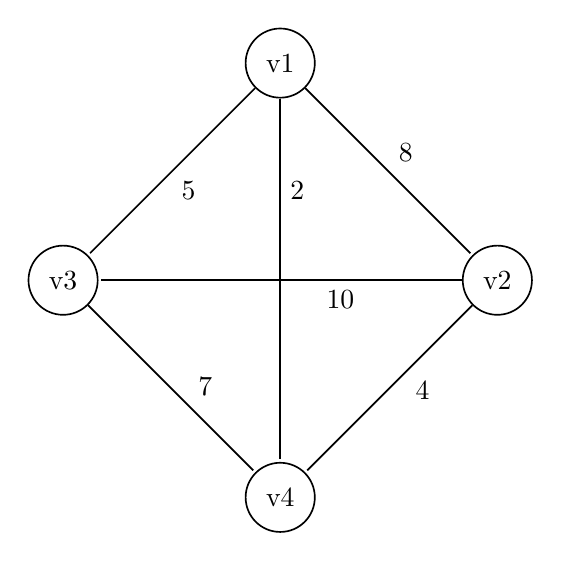
\begin{tikzpicture}[
    > = , % arrow head style
    shorten > = 1pt, % don't touch arrow head to node
    auto,
    node distance = 3cm, % distance between nodes
    semithick % line style
    ]

    \tikzset{every state}=[
    draw = black,
    thick,
    fill = white,
    minimum size = 1mm
    ]

    \node[state] (v1) {v1};
    \node[state] (v2) [below right=of v1] {v2};
    \node[state] (v3) [below left=of v1] {v3};
    \node[state] (v4) [below right=of v3] {v4};
  
    \path[->] (v1) edge  node[] {8} (v2);
    \path[->] (v1) edge  node[pos=0.5,below right] {5} (v3);
    \path[->] (v1) edge  node[pos=0.2,below right] {2} (v4);
    \path[->] (v2) edge  node[pos=0.4,below right] {10} (v3);
    \path[->] (v2) edge  node[pos=0.4,below right] {4} (v4);
    \path[->] (v3) edge  node[pos=0.6,above right] {7} (v4);
    \end{tikzpicture}

Then using definition \ref{Hamiltonian Cycle} the distinct Hamiltonian Cycles in G are (Hamiltonian Cycles not using the exact same edges) :\\
1. (v1 v3 v4 v2 v1) with cost 24\\
2. (v1 v3 v2 v4 v1) with cost 21\\
3. (v1 v2 v3 v4 v1) with cost 27\\
Thus using definition \ref{Travelling Salesman Problem}, the answer for the Travelling Salesman Problem on this graph instance would be (v1 v3 v2 v4 v1), because it is the minimum weight Hamiltonian Cycle in G.
\newpage
After illustrating the Travelling Salesman Problem, some basic results are needed to be prooved so that no assumptions are taken.In fact ,definition \ref{Travelling Salesman Problem} suggests that in the Travelling Salesman Problem it is already known that the graph to be evaluated is Hamiltonian, otherwise a minimum weight Hamiltonian Cycle can never be found.This uncertainty can be tackled by proving that any complete graph on more than 3 vertices is Hamiltonian. This fact is proved in lemma \ref{Kn is Hamiltonian} below.
\begin{lemma}
\label{Kn is Hamiltonian}
For n $\geq$ 3, The complete graph on n vertices is Hamiltonian
\end{lemma}
\begin{proof}
Let $K_n$ be the complete graph on n $\geq$ 3 vertices labelled v1,v2,...,vn. Order all the vertices in the order v1,v2,...,vn with no repetitions of vertices.Then C=(v1 v2 ... vn v1) must be a cycle in $K_n$ because because $\forall$ vi,vj $\in$ C, vi $\ne$ vj then $\{vi,vj\}$ $\in$ E($K_n$). Also since $\forall$ v $\in$ V($K_n$) ,v is a vertex in the cycle with only one occurence in C(except for v1 which has 2 occurences) then C must be a Hamiltonian Cycle in $K_n$ . Thus $K_n$ must be Hamiltonian.
\end{proof}
Since every $K_n$ for n $\geq$ 3 vertices is Hamiltonian this suggests that in order to find the minimum weight Hamiltonian cycle one could compute every Hamiltonian cycle in $K_n$ and then return the cycle of least cost. However, this is infeasible because this algorithm $K_n$ generates $\frac{(n-1)!}{2}$ distinct Hamiltonian cycles(proved in  lemma $\ref{running_time}$ below) . Thus the algorithm would have a time complexity O(n!) making it very infeasible to compute in reasonable time.\cite{geeksforgeeks_2018}
\begin{lemma}
\label{running_time}
For n $\geq$ 3 the complete graph on n vertices has $\frac{(n-1)!}{2}$ distinct Hamiltonian cycles
\end{lemma}
\begin{proof}
Let $K_n$ be the complete graph on n $\geq$ 3 vertices .Since E($K_n$) contains an edge for every possible dinstinct vertices u,v $\in$ V($K_n$) then every permutation of V($K_n$) must represent a Hamiltonian Cycle in $K_n$ and vice versa(1-1 correspondence). Now on n vertices there are n! possible number of permutations, thus we have n! Hamiltonian cycles due to the 1-1 correspondence. However, different permutations of V($K_n$ ) may represent the same Hamiltonian Cycle in $K_n$, since the same edges would be used from E($K_n$) but in a different order of the vertices . In fact, consider the Hamiltonian Cycle C represented by the permutation (v1 v2...vn). In terms of Hamiltonian cycles, the permutation (v1 v2 ...vn) is the same as the permutation (v2...vn v1) because the same edges in E($K_n$) are used . Thus for each Hamiltonian cycle in $K_n$ we can have n permutations representing the same cycle.However,for each of these n permutation representations , the reverse of each of the permutations represent the same Hamiltonian Cycle with the difference being that the cycle is traversed in reverse order, thus we have 2n permutations representing the same Hamiltonian Cycle. Thus the number of distinct permutations is $\frac{n!}{2n}$ = $\frac{(n-1)!}{2}$. \cite{mathematics_stack_exchange_2012}
\end{proof}
Lemma \ref{running_time} confirms the difficulty in writing an algorithm that executes in reasonable time, to solve the Travelling Salesman Problem for any number of cities .The reason is that in order to compute the minimum weight Hamiltonian Cycles , all algorithms that were constructed so far take superpolynomial time. This leads to a discussion on the different classes of problems including NP-Completness in the next sub-section.
\subsection{The classes P,NP and NPC}
It is known that not all problems in the universe can be solved by algorithms even if a lot of time is dedicated to them . In fact Alan Turing proved this by proposing the Halting problem which is a problem that proveably cannot be solved by any computer. In addition to this class of problems there is the class of NP-Complete problems(NPC). For problems in this class, no polynomial time algorithm has yet been discovered , but at the same time no one was able to prove that such a polynomial time algorithm exists or not for them. In what follows, the important classes of problems will be discussed more formally, describing in the process how to prove that a problem is in NPC so that it can be proved that TSP is NP-Complete. \cite{geeksforgeeks_2018_2}\\
\\
The three most important classes of problems are called P,NP and NP-Complete (NPC). Firstly, problems belonging to P are problems that can be solved in polynomial time and thus are tractable. Such problems can be solved by algorithms that can complete their execution in a reasonible time. Secondly, the class NP consists of decision problems that can be verified in polynomial time . This means that given a certificate(answer) to a problem in NP , this certificate can be checked in polynomial time to verify if it is correct or not. Thirdly, a decision problem is in the class NPC if it is in NP and it is as hard as any problem in NP(this will be made more clear in the next paragraph when discussing how to compare problems' complexity using reductions). Thus when proving that a problem is NP-Complete a statement is being made as to how hard is that problem and thus that no efficient algorithm exists. It must be noted that according to the definitions , in order to be in the classes NP and NPC the problems must be decision problems. This is of great benefit because decision problems are much easier to reason about and all problems in the universe can be converted to a decision problem representing and vice versa.For example, TSP can be converted to the decision problem, "Is there a Hamiltonian cycle in $K_n$ having length less than k?". \cite{cormen_leiserson_rivest_stein}\\
\\
Thus reasoning on whether a problem is as hard as any other problem, is as hard as conducting the same reasoning on their decision versions. Checking whether a decision problem is as hard as another decision problem can be done using reduction algorithms. Suppose that 2 decision problems A and B are given, were $\alpha$ is the input to the decision problem A and $\beta$ is the input to decision problem B. Then a reduction algorithm transforms any input $\alpha$ of A into some input $\beta$ of B such that the transformation takes polynomial time and the answers are the same. This means the answer for the decision problem A given $\alpha$ is 'yes' $\iff$ the answer for the decision problem B given $\beta$ is 'yes'. Thus if a decision problem A is required to be solved in polynomial time and it is known that a decision problem B can be solved in polynomial time , then A can be solved in polynomial time if a reduction algorithm can transform every input of A to and input of B since transforming this instance would take polynomial time and runnning the algorithm on this transformed instance takes also polynomial time . Thus the total number of time is polynomial . Note that this could only be done if one problem can be transformed into an other , since it is only then that 'yes' result for one is a 'yes' result for the other. \cite{cormen_leiserson_rivest_stein}\\
\\
Read geek for geeks to join everything and explain as least as hard in np	

\newpage
\section{Conclusion}
\newpage
\bibliography{bibliography}
\bibliographystyle{IEEEtran}
\end{document}